%% =====================================================================
% Capítulo: Escenario 1 -- fuga de información mediante correo electrónico
% Misma estructura que el escenario USB (03_3_desarrollo_usb.tex):
% planteamiento, preparación, cadena de custodia, adquisición, análisis
% y conclusiones. Usa lo que define estilo_pericial.sty (listados con
% style=terminal y tablas con booktabs y caption).
%
% Los datos de la cadena de custodia proceden de los metadatos de los
% ficheros del propio laboratorio (carpeta IFOR_CASO_CORREO) y de las
% capturas realizadas durante la simulación.
% =====================================================================

% Código en línea (admite _, $, ^, {}, <, > ... sin escapar). Se vuelve a
% declarar por si este capítulo se compila solo con \includeonly.
\providecommand{\cod}[1]{\texttt{\detokenize{#1}}}

\subsection{Escenario 1: fuga de información mediante correo electrónico}
\label{cap:correo}

En este capítulo se documenta el primero de los escenarios del enunciado: la
fuga del fichero \cod{Confidencial.pdf} del \textit{Windows Server} 2008 hacia
un destinatario externo mediante correo electrónico. El correo se envía entre
dos miembros del grupo y el estudio y la documentación de la evidencia los
realiza uno solo de ellos. El trabajo consiste en reproducir la extracción,
recibir una imagen del equipo desde el que se envió el mensaje, adquirirla
sin modificarla y mantener la cadena de custodia.

% ---------------------------------------------------------------------
\subsection{Planteamiento y alcance}
El enunciado plantea una fuga en la que el fichero se saca del servidor y se
envía por correo electrónico. Para poder reproducirla de forma aislada, el
grupo desplegó un servicio de correo propio (descrito en el apartado anterior)
y simuló el incidente en dos máquinas virtuales. Se supone después que el
director de la empresa, Jaime Diez Zurro, entrega al grupo la imagen del disco
del equipo desde el que se realizó el envío.

Quedan fuera de este escenario los otros dos medios de extracción (Dropbox y
dispositivo USB), que se tratan en sus propios apartados.

\begin{itemize}
  \item \textbf{Origen:} \cod{Confidencial.pdf} en el \textit{Windows Server}
        2008 configurado en la entrega anterior.
  \item \textbf{Soporte a analizar:} el disco virtual (\cod{.vdi}) del equipo
        cliente \textit{Windows} 11, desde el que se envió el mensaje.
  \item \textbf{Entregable:} imagen del disco, cadena de custodia,
        informe de pruebas (mensaje, adjunto y registros del servidor de
        correo) y conclusiones.
  \item \textbf{Perito encargado:} \PeritoDos.
\end{itemize}

% ---------------------------------------------------------------------
\subsection{Preparación del escenario}
\label{sec:correo-preparacion}
A continuación se detallan la arquitectura de red desplegada, la extracción del
documento y el envío por correo, con la fecha y hora de cada paso.

\subsubsection{Arquitectura de red y sistemas implicados}
Se han desplegado dos máquinas virtuales en el mismo segmento de red local
(\cod{192.168.255.0/24}), con puerta de enlace en \cod{192.168.255.1}:

\begin{itemize}
    \item \textbf{Servidor corporativo (\textit{Windows Server}, WS):}
    repositorio de la información sensible, con la dirección IPv4
    \cod{192.168.255.6} (figura~\ref{fig:ip-ws}).
    \item \textbf{Equipo cliente (\textit{Windows} 11, W11):} estación desde la
    que se realiza la extracción y el envío, con la dirección IPv4
    \cod{192.168.255.5} (figura~\ref{fig:ip-w11}).
\end{itemize}

\begin{figure}[H]
    \centering
    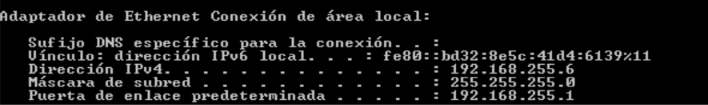
\includegraphics[width=0.85\textwidth]{Recursos/ip_WS.png}
    \caption{Configuración de red del servidor (\cod{192.168.255.6}).}
    \label{fig:ip-ws}
\end{figure}

\begin{figure}[H]
    \centering
    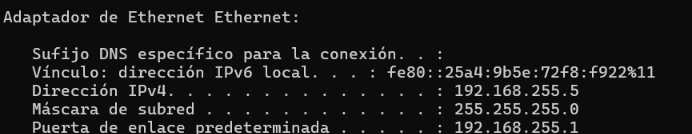
\includegraphics[width=0.85\textwidth]{Recursos/ip_pc_ladron.png}
    \caption{Configuración de red del equipo cliente (\cod{192.168.255.5}).}
    \label{fig:ip-w11}
\end{figure}

\subsubsection{Recurso compartido y extracción del documento}
El vector inicial es un recurso compartido SMB (\textit{Server Message Block})
del servidor. Para publicarlo, en las propiedades de la carpeta se activó
\textit{Compartir esta carpeta} con el nombre \cod{ConfidencialInfo}, se
asignaron los permisos de red al usuario autorizado y se comprobó que los
permisos locales NTFS le permitían el acceso, ya que Windows aplica siempre la
intersección más restrictiva de ambos. El comando \cod{net share} confirma la
publicación del recurso, asociado a la carpeta local \cod{C:\ConfidencialInfo}
(figura~\ref{fig:carpeta-compartida}).

\begin{figure}[H]
    \centering
    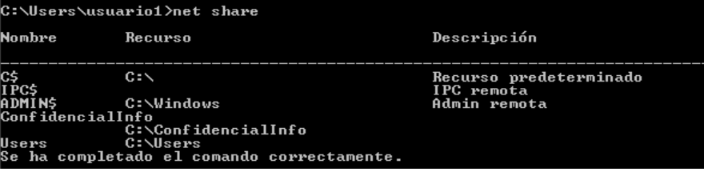
\includegraphics[width=0.85\textwidth]{Recursos/carpeta_compartida_WS.png}
    \caption{Recursos compartidos del servidor, con \cod{ConfidencialInfo}.}
    \label{fig:carpeta-compartida}
\end{figure}

Antes de la extracción se calculó la huella SHA-256 del fichero en el servidor
con \cod{certutil} (figura~\ref{fig:hash-ws}), para poder demostrar después
que la copia es idéntica al original.

\begin{figure}[H]
    \centering
    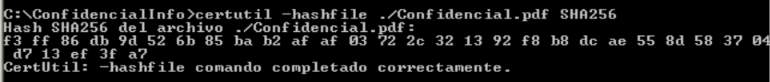
\includegraphics[width=0.85\textwidth]{Recursos/confidencial_en_WS_hash.png}
    \caption{Huella SHA-256 de \cod{Confidencial.pdf} en el servidor.}
    \label{fig:hash-ws}
\end{figure}

Desde el equipo cliente se accedió al recurso mediante su ruta UNC
(\textit{Universal Naming Convention}), sin asignar letra de unidad:

\begin{lstlisting}[style=terminal,breaklines=true]
explorer \\192.168.255.6\ConfidencialInfo
\end{lstlisting}

El fichero se copió a \cod{C:\Evidencias\Confidencial.pdf} en el equipo
cliente y se verificó con \cod{Get-FileHash} que su huella coincide con la del
servidor (figura~\ref{fig:hash-w11}).

\begin{figure}[H]
    \centering
    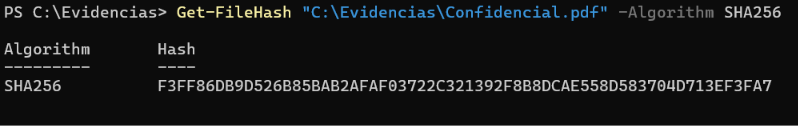
\includegraphics[width=0.85\textwidth]{Recursos/confidencial_en_Windows11_hash.png}
    \caption{Verificación con \cod{Get-FileHash} en \textit{Windows} 11 tras la
    extracción.}
    \label{fig:hash-w11}
\end{figure}

\subsubsection{Envío por correo electrónico}
Para no depender de servicios de terceros se empleó el servicio de correo
propio, con dos buzones: \cod{pepe@empresa.local} (origen, asociado al empleado)
y \cod{ana@empresa.local} (destino). Desde el equipo cliente se redactó un
mensaje de asunto <<Envío Confidencial>> dirigido a \cod{ana@empresa.local} con
\cod{Confidencial.pdf} como adjunto. El servidor lo procesó de forma interna y
lo depositó en el buzón de destino, sin que el tráfico saliera del laboratorio.
La figura~\ref{fig:correo-registrado} muestra el mensaje recibido en el
webmail: remitente, destinatario, fecha (martes 10 de noviembre de 2026,
18:26:34, hora \cod{+0100}) y el adjunto.

\begin{figure}[H]
    \centering
    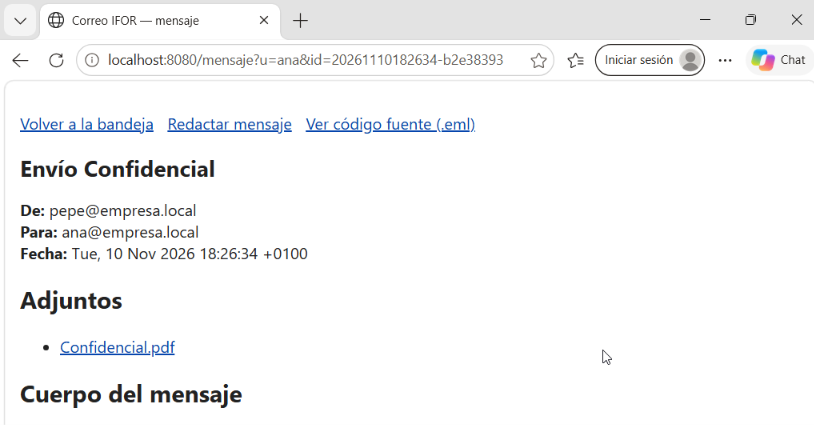
\includegraphics[width=0.85\textwidth]{Recursos/correo_registrado.png}
    \caption{Mensaje recibido en el buzón de \cod{ana@empresa.local}.}
    \label{fig:correo-registrado}
\end{figure}

% ---------------------------------------------------------------------
\subsection{Cadena de custodia}
\label{sec:correo-custodia}
Tras la simulación (10 de noviembre de 2026), la máquina virtual del equipo
cliente se apagó y su disco virtual, \cod{Maquina_Corrreo.vdi}, quedó como la
imagen de disco de este escenario. Conforme al supuesto del enunciado, el
director de la empresa, Jaime Diez Zurro, entrega al grupo esta imagen
\textbf{junto con la clave de recuperación de BitLocker}, sin la cual el
contenido del volumen del sistema no es legible (véase el apartado
\ref{sec:correo-bitlocker}). El peritaje de este escenario lo realiza
\PeritoDos, que es quien custodia el soporte.

Las fechas y horas de la tabla proceden de los metadatos del propio fichero
\cod{.vdi} en el equipo de análisis (última modificación, creación de la copia
y último acceso), de la creación de la captura con el \textit{hash} y de los
registros de la fase de análisis. No se precintó el soporte ni se calculó
ningún \textit{hash} antes del que se indica en la tabla, por lo que el estado
de la imagen queda fijado por ese cálculo. Todas las horas están en hora local
(CET, UTC+1).

\begin{table}[H]
\centering
\small
\renewcommand{\arraystretch}{1.3}
\begin{tabular}{@{}p{0.22\textwidth}p{0.13\textwidth}p{0.13\textwidth}p{0.43\textwidth}@{}}
\toprule
\textbf{Fecha y hora} & \textbf{Entrega} & \textbf{Recibe} & \textbf{Motivo y observaciones} \\
\midrule
10/11/2026, de 17:07 a 18:35 & -- & \PeritoDos &
Simulación de la fuga en las máquinas virtuales: configuración de red,
extracción desde el servidor y comprobación de huellas. El mensaje se envía a
las 18:26:34. \\
12/11/2026, 20:46:41 & -- & \PeritoDos &
Última modificación del disco virtual \cod{Maquina_Corrreo.vdi}: es la última
vez que la máquina virtual escribió en él. \\
12/11/2026, 20:52 & Jaime Diez Zurro (supuesto) & \PeritoDos &
Entrega de la imagen y de la clave de recuperación de BitLocker (protector
\cod{{04D7EFA5-4921-4EFD-8F65-7D2AAF4DF62A}}) al grupo para el peritaje, según
el supuesto del enunciado. Entrega simulada: el disco ya obraba en poder del
perito. La copia en la carpeta \cod{IFOR_CASO_CORREO} se creó a las 20:52:06. \\
12/11/2026, 20:59 & \PeritoDos & \PeritoDos (perito) &
Cálculo del primer \textit{hash} (SHA-256) de la imagen. \\
24/11/2026, hasta las 00:02 & \PeritoDos (perito) & \PeritoDos &
Se crea una copia de trabajo de la imagen y se comprueba que su \textit{hash}
es idéntico al del original. Después se cambia el identificador (UUID) de la
copia, para poder registrarla en \textit{VirtualBox}. \\
24/11/2026, de 00:05 a 00:48 & \PeritoDos (perito) & \PeritoDos &
Análisis en la máquina virtual \textit{Kali Linux}, con la copia de trabajo
conectada como disco inmutable. Cálculo del \textit{hash} del disco completo
al empezar y al terminar. \\
24/11/2026, 00:49 & \PeritoDos (perito) & \PeritoDos &
Recálculo de los \textit{hash} del original y de la copia. Custodia en el
equipo del perito, en la carpeta \cod{IFOR_CASO_CORREO}, sin modificar. \\
\bottomrule
\end{tabular}
\caption{Registro de custodia de la imagen del equipo cliente.}
\label{tab:correo-custodia}
\end{table}

% ---------------------------------------------------------------------
\subsection{Adquisición de la evidencia}
\label{sec:correo-adquisicion}

\subsubsection{Imagen utilizada}
Dado que el entorno completo se montó en \textit{VirtualBox}, el disco virtual
del equipo cliente puede utilizarse directamente como imagen del disco del
atacante interno. No se creó una imagen RAW con una herramienta de adquisición:
se trabaja sobre el propio \cod{.vdi}, que es un contenedor de disco virtual de
VirtualBox (no una copia bit a bit del soporte físico).

\begin{table}[H]
\centering
\small
\renewcommand{\arraystretch}{1.3}
\begin{tabular}{@{}p{0.34\textwidth}p{0.62\textwidth}@{}}
\toprule
\textbf{Parámetro} & \textbf{Valor} \\
\midrule
Fichero de imagen & \cod{Maquina_Corrreo.vdi} \\
Ubicación & \cod{C:\Users\hugop\Desktop\IFOR_CASO_CORREO} \\
Formato & Disco virtual VirtualBox (\cod{.vdi}) \\
Tamaño del fichero & 39.403.388.928 bytes (unos 36,7 GiB) \\
Tamaño del disco virtual & 85.899.345.920 bytes (80 GiB) \\
Última modificación & 12/11/2026, 20:46:41 \\
Creación de la copia & 12/11/2026, 20:52:06 \\
Copia de trabajo & \cod{copia_trabajo\Maquina_Corrreo_trabajo.vdi} \\
Equipo de análisis & \textit{Windows} 11 (compilación 26200) \\
Herramienta de cálculo & \cod{Get-FileHash} (\textit{PowerShell}) \\
\bottomrule
\end{tabular}
\caption{Parámetros de la imagen del equipo cliente.}
\label{tab:correo-imagen}
\end{table}

\subsubsection{Verificación de integridad}
Se calculó la huella SHA-256 de la imagen con la misma herramienta nativa de
\textit{Windows} que se había utilizado para el resto de ficheros
(figura~\ref{fig:correo-hash-imagen}). Se recalculó el 24 de noviembre de 2026,
al terminar el análisis, y el valor coincide con el de la captura, lo que
acredita que la imagen original no se modificó.

\begin{lstlisting}[style=terminal,breaklines=true]
Get-FileHash -Path "C:\Users\hugop\Desktop\IFOR_CASO_CORREO\Maquina_Corrreo.vdi" -Algorithm SHA256
SHA-256: 85EBDF723060F36E7E8EF4A6B848D85BFC2DB6B4B1597A51E13F676A193898A6
\end{lstlisting}

\begin{figure}[H]
    \centering
    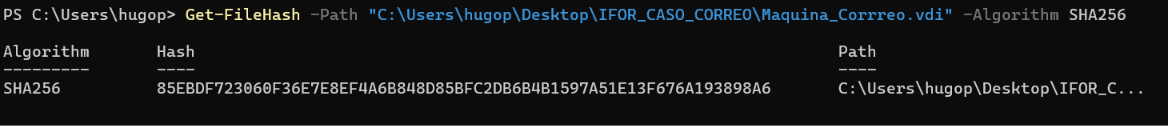
\includegraphics[width=0.85\textwidth]{Recursos/imagen_disco_correo.png}
    \caption{Huella SHA-256 de la imagen del disco del equipo cliente.}
    \label{fig:correo-hash-imagen}
\end{figure}

El análisis no se hace sobre el original, sino sobre una \textbf{copia de
trabajo}. Para poder registrarla en \textit{VirtualBox} (que no admite dos
discos con el mismo identificador) hubo que cambiarle el UUID, y ese cambio
modifica unos bytes de la cabecera del fichero. Por eso el \textit{hash} del
fichero de la copia ya no coincide con el del original. La comparación
relevante es la del \textbf{contenido}: el \textit{hash} de la copia justo
antes del cambio es idéntico al del original, y el \textit{hash} del disco
completo, visto desde \textit{Kali} (\cod{sha256sum /dev/sdb}), es el mismo al
empezar y al terminar el análisis (tabla~\ref{tab:correo-hashes}).

\begin{table}[H]
\centering
\footnotesize
\renewcommand{\arraystretch}{1.3}
\begin{tabular}{@{}p{0.34\textwidth}p{0.10\textwidth}p{0.50\textwidth}@{}}
\toprule
\textbf{Elemento} & \textbf{Alg.} & \textbf{Hash} \\
\midrule
Original \cod{.vdi} (12/11/2026) & SHA-256 & \cod{85EBDF723060F36E7E8EF4A6B848D85B}\newline
\cod{FC2DB6B4B1597A51E13F676A193898A6} \\
Original \cod{.vdi} (24/11/2026) & SHA-256 & \cod{85EBDF723060F36E7E8EF4A6B848D85B}\newline
\cod{FC2DB6B4B1597A51E13F676A193898A6} \\
Copia de trabajo, antes de cambiar el UUID & SHA-256 & \cod{85EBDF723060F36E7E8EF4A6B848D85B}\newline
\cod{FC2DB6B4B1597A51E13F676A193898A6} \\
Copia de trabajo, tras cambiar el UUID & SHA-256 & \cod{AE25F5C373F6834E914ADBBCA9776FDF}\newline
\cod{A6935678E946248054F4FB85F1CDE1E2} \\
Disco completo en \textit{Kali} (inicio) & SHA-256 & \cod{d97ac1ddf9f650ffb35b1ea757e5756a}\newline
\cod{29582980fcb006843321d78a2936e714} \\
Disco completo en \textit{Kali} (final) & SHA-256 & \cod{d97ac1ddf9f650ffb35b1ea757e5756a}\newline
\cod{29582980fcb006843321d78a2936e714} \\
\bottomrule
\end{tabular}
\caption{Verificación de integridad de la imagen y de la copia de trabajo.}
\label{tab:correo-hashes}
\end{table}

\noindent\textbf{Importante.} La imagen original se conserva sin modificar, con
su \textit{hash} registrado en la cadena de custodia. Todo el examen se hace
sobre la copia, sin arrancar nunca la máquina virtual original, porque al
iniciarse modificaría el \cod{.vdi}.

\subsubsection{Entorno y herramientas de análisis}
\label{sec:correo-herramientas}
El análisis se realizó en la máquina virtual \textit{Kali Linux} 2025.3
(núcleo 6.12.38), a la que se conectó la copia de trabajo como disco
\textbf{inmutable}: \textit{VirtualBox} no permite disco duro de solo lectura,
y el modo inmutable envía cualquier escritura a un fichero aparte sin tocar la
copia. Además, dentro de \textit{Kali} se activó el bloqueo de escritura del
disco (\cod{blockdev --setro}, resultado \cod{1}). Se emplearon las
herramientas de la tabla~\ref{tab:correo-herramientas}, todas estándar y
libres. Las órdenes y las salidas completas se conservan en la carpeta de
evidencias.

\begin{table}[H]
\centering
\small
\renewcommand{\arraystretch}{1.3}
\begin{tabular}{@{}p{0.24\textwidth}p{0.14\textwidth}p{0.54\textwidth}@{}}
\toprule
\textbf{Herramienta} & \textbf{Versión} & \textbf{Uso} \\
\midrule
\cod{fdisk}, \cod{mmls} & \textit{TSK} 4.12.1 & Tabla de particiones del disco \\
\cod{cryptsetup bitlkDump} & 2.8.1 & Lectura de los metadatos de BitLocker \\
\cod{dislocker} & 0.7.4 & Descifrado de BitLocker en solo lectura con la clave de recuperación \\
\cod{fsstat}, \cod{fls}, \cod{istat}, \cod{icat} & \textit{TSK} 4.12.1 & Examen del sistema de ficheros NTFS: listado, metadatos y extracción \\
\cod{mactime} & \textit{TSK} 4.12.1 & Línea temporal \\
\cod{md5sum}, \cod{sha1sum}, \cod{sha256sum} & coreutils & Huellas de integridad \\
\bottomrule
\end{tabular}
\caption{Herramientas utilizadas en \textit{Kali Linux}.}
\label{tab:correo-herramientas}
\end{table}

\subsubsection{Estructura del disco y cifrado BitLocker}
\label{sec:correo-bitlocker}
El disco usa tabla de particiones GPT con cuatro particiones
(tabla~\ref{tab:correo-particiones}). La partición del sistema (\cod{C:}) está
\textbf{cifrada con BitLocker}: su primer sector no contiene la firma de NTFS
sino la de BitLocker (\cod{-FVE-FS-}), por lo que sin la clave el contenido no
es legible. Es lo habitual en equipos con \textit{Windows} 11, que activa el
cifrado de dispositivo de forma predeterminada.

\begin{table}[H]
\centering
\small
\renewcommand{\arraystretch}{1.3}
\begin{tabular}{@{}p{0.07\textwidth}p{0.18\textwidth}p{0.20\textwidth}p{0.45\textwidth}@{}}
\toprule
\textbf{N.º} & \textbf{Sector inicial} & \textbf{Sectores} & \textbf{Contenido} \\
\midrule
1 & 2.048 & 409.600 & Partición del sistema EFI (200 MB) \\
2 & 411.648 & 32.768 & Reservada de Microsoft (16 MB) \\
3 & 444.416 & 165.470.208 & Volumen \cod{C:}, cifrado con BitLocker (78,9 GB) \\
4 & 165.914.624 & 1.853.440 & Entorno de recuperación de Windows (905 MB) \\
\bottomrule
\end{tabular}
\caption{Particiones del disco del equipo cliente (sectores de 512 bytes).}
\label{tab:correo-particiones}
\end{table}

Los metadatos de BitLocker (figura~\ref{fig:correo-kali-bitlocker}) indican
que el volumen se creó el 9 de noviembre de 2026, con la descripción
\cod{DESKTOP-DI359N9 C: 09/11/2026}, y que usa el cifrado \textbf{AES-XTS de
128 bits}. Tiene dos protectores de la clave maestra: una \textit{clave de
recuperación} (identificador \cod{04d7efa5-4921-4efd-8f65-7d2aaf4df62a}) y una
\textit{clave en claro}. Esta última es la que Windows deja cuando el cifrado
está \textbf{suspendido}: en ese estado la clave queda accesible para el
propio sistema.

\begin{figure}[H]
    \centering
    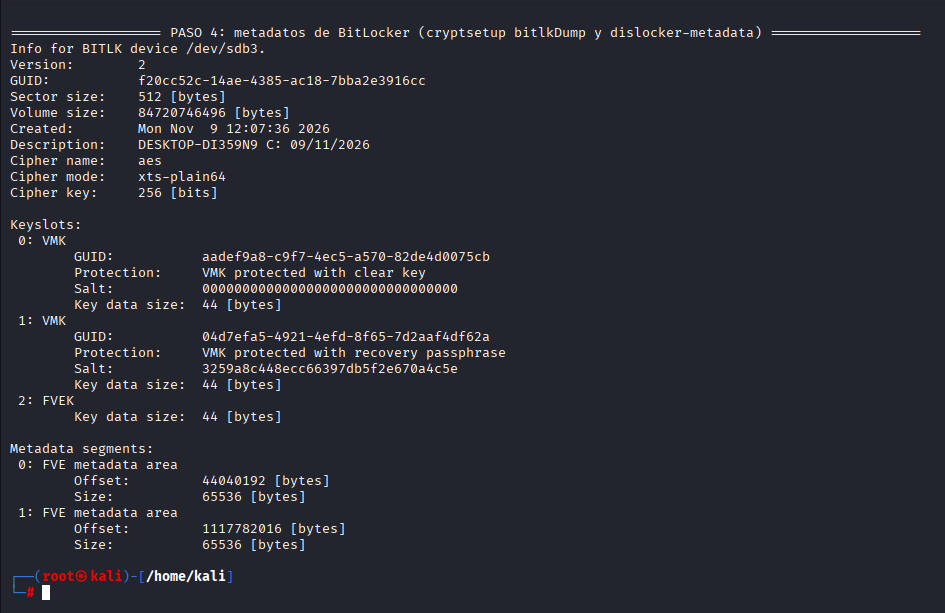
\includegraphics[width=0.85\textwidth]{Recursos/correo_kali_bitlocker.png}
    \caption{Metadatos de BitLocker del volumen \cod{C:} (\cod{cryptsetup bitlkDump}).}
    \label{fig:correo-kali-bitlocker}
\end{figure}

Conforme al supuesto del enunciado, la clave de recuperación la facilita el
director de la empresa junto con el equipo (véase la
tabla~\ref{tab:correo-custodia}). Con ella se descifró el volumen en solo
lectura:

\begin{lstlisting}[style=terminal,breaklines=true]
dislocker -V /dev/sdb3 -p<clave de recuperacion> -r -- /mnt/bitlocker
\end{lstlisting}

\textit{dislocker} presenta el volumen en claro como un fichero
(\cod{dislocker-file}) que \textit{The Sleuth Kit} reconoce como NTFS, con
259.073 entradas en la \cod{\$MFT} (figura~\ref{fig:correo-kali-dislocker}).
Se probó antes con \cod{cryptsetup bitlkOpen}, pero esta herramienta no
admite volúmenes con la clave en claro (cifrado suspendido), por lo que se
utilizó \textit{dislocker}. La clave de recuperación no se reproduce en este
informe.

\begin{figure}[H]
    \centering
    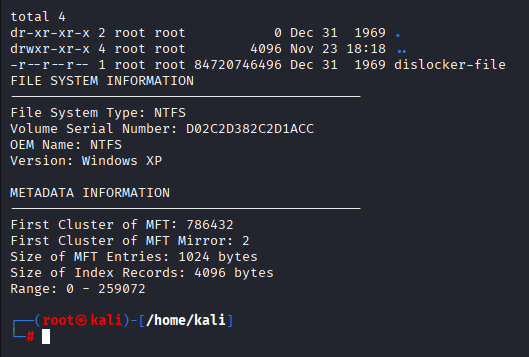
\includegraphics[width=0.6\textwidth]{Recursos/correo_kali_dislocker.png}
    \caption{Volumen descifrado y reconocido como NTFS (\cod{fsstat}).}
    \label{fig:correo-kali-dislocker}
\end{figure}

% ---------------------------------------------------------------------
\subsection{Informe de pruebas}
\label{sec:correo-analisis}

En el volumen \cod{C:} descifrado se localizó el servidor de correo del grupo,
en \cod{C:\Users\hugop\Downloads\IFOR_P2-main\IFOR_P2-main\servidor}, junto
con los tres elementos que genera por cada envío (mensaje, adjunto y registro).
Se obtuvo el listado de ficheros con \cod{fls}, se consultaron sus metadatos con
\cod{istat} y se extrajeron con \cod{icat}, calculando su MD5, SHA-1 y SHA-256.

\textbf{Nota sobre las horas.} Las marcas temporales de NTFS están en UTC.
\cod{istat} las muestra en la zona horaria de \textit{Kali} (EST, UTC$-$5) y
\cod{mactime} se ejecutó en UTC. En este informe se convierten a hora local
(CET, UTC+1): 17:26:34 UTC (12:26:34 EST) son las 18:26:34 de la hora del
mensaje.

\subsubsection{Prueba 1: mensaje \cod{.eml}}
Se trata del fichero
\cod{servidor\buzones\ana\mensajes\20261110182634-b2e38393.eml} (entrada 226668 de
la \cod{\$MFT}, activa, 920 bytes). Su contenido, sin alterar, es:

\begin{lstlisting}[style=terminal,basicstyle=\ttfamily\footnotesize,breaklines=true]
Received: from webmail (127.0.0.1)
	by empresa.local (servidor IFOR) with HTTP;
	Tue, 10 Nov 2026 18:26:34 +0100
From: pepe@empresa.local
To: ana@empresa.local
Subject: =?utf-8?q?Env=C3=ADo?= Confidencial
Date: Tue, 10 Nov 2026 18:26:34 +0100
Message-ID: <179433159411.4376.15980925307143410306@DESKTOP-DI359N9>
Content-Type: multipart/mixed; boundary="===============1681336223577990369=="
...
Content-Type: application/pdf
Content-Transfer-Encoding: base64
Content-Disposition: attachment; filename="Confidencial.pdf"
\end{lstlisting}

\begin{table}[H]
\centering
\small
\renewcommand{\arraystretch}{1.3}
\begin{tabular}{@{}p{0.28\textwidth}p{0.68\textwidth}@{}}
\toprule
\textbf{Campo} & \textbf{Valor} \\
\midrule
Remitente (\cod{From}) & \cod{pepe@empresa.local} \\
Destinatario (\cod{To}) & \cod{ana@empresa.local} \\
Asunto & Envío Confidencial \\
Fecha (\cod{Date}) & Tue, 10 Nov 2026 18:26:34 +0100 \\
\cod{Received} & de \cod{webmail (127.0.0.1)}, por \cod{empresa.local} (servidor IFOR), con \cod{HTTP} \\
Identificador del mensaje & \cod{<179433159411.4376.}\newline\cod{15980925307143410306@DESKTOP-DI359N9>} \\
Adjunto & \cod{Confidencial.pdf} (\cod{application/pdf}, base64) \\
SHA-256 del \cod{.eml} & \cod{1446aec75726e0bc745898a4055316e6}\newline
\cod{65cf52840236b520b16c3c315c8b2fd9} \\
\bottomrule
\end{tabular}
\caption{Cabeceras y huella del mensaje recuperado.}
\label{tab:correo-cabeceras}
\end{table}

La cabecera \cod{Received} indica que el mensaje entró por el \textit{webmail}
desde la dirección local \cod{127.0.0.1}, es decir, desde la propia máquina
donde se ejecuta el servidor. La hora de la cabecera \cod{Date} coincide con la
captura del \textit{webmail} (figura~\ref{fig:correo-registrado}).

\begin{figure}[H]
    \centering
    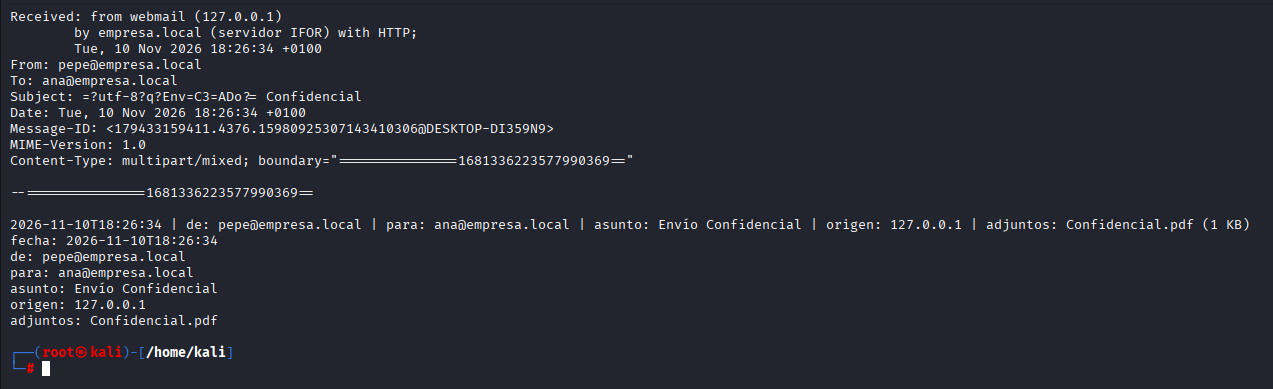
\includegraphics[width=0.9\textwidth]{Recursos/correo_kali_eml_logs.png}
    \caption{Mensaje, registro de envíos y fichero \cod{envio.txt} extraídos.}
    \label{fig:correo-kali-eml}
\end{figure}

\subsubsection{Prueba 2: adjunto y comparación con el original}
El adjunto aparece en tres puntos de la imagen (tabla~\ref{tab:correo-adjuntos}):
decodificado del propio \cod{.eml} (el 	extit{Base64} se decodificó con 	extit{PowerShell}), extraído por el servidor al buzón de
destino y guardado en la carpeta de copias de envío. A ello se suma la copia de
origen en el equipo cliente, \cod{C:\Evidencias\Confidencial.pdf}. Los cuatro
ficheros son de 103 bytes y tienen el \textbf{mismo SHA-256 que el original}
calculado en el servidor (\cod{f3ff86db\ldots3fa7}). Su contenido es un texto
breve en el que el gerente de la empresa indica que se trata de información
confidencial, igual que en los demás escenarios.

\begin{table}[H]
\centering
\footnotesize
\renewcommand{\arraystretch}{1.3}
\begin{tabular}{@{}p{0.30\textwidth}p{0.66\textwidth}@{}}
\toprule
\textbf{Fichero (entrada \cod{\$MFT})} & \textbf{SHA-256} \\
\midrule
Original en el servidor (certutil) & \cod{f3ff86db9d526b85bab2afaf03722c32}\newline
\cod{1392f8b8dcae558d583704d713ef3fa7} \\
Adjunto decodificado del \cod{.eml} & \cod{f3ff86db9d526b85bab2afaf03722c32}\newline
\cod{1392f8b8dcae558d583704d713ef3fa7} \\
\cod{buzones\ana\adjuntos\...} (226671) & \cod{f3ff86db9d526b85bab2afaf03722c32}\newline
\cod{1392f8b8dcae558d583704d713ef3fa7} \\
\cod{adjuntos_enviados\...} (226675) & \cod{f3ff86db9d526b85bab2afaf03722c32}\newline
\cod{1392f8b8dcae558d583704d713ef3fa7} \\
\cod{C:\Evidencias\Confidencial.pdf} (234421) & \cod{f3ff86db9d526b85bab2afaf03722c32}\newline
\cod{1392f8b8dcae558d583704d713ef3fa7} \\
\bottomrule
\end{tabular}
\caption{Comparación del adjunto con el original. Coinciden todos.}
\label{tab:correo-adjuntos}
\end{table}

El MD5 del adjunto, \cod{4c9283480e5692410e177df58323e732}, coincide también
con el que \textit{Autopsy} muestra para el fichero del escenario de
\textit{Dropbox}, lo que confirma que es el mismo documento en los tres
escenarios.

\begin{figure}[H]
    \centering
    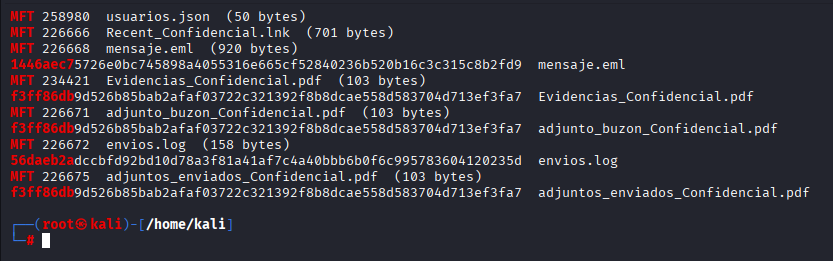
\includegraphics[width=0.9\textwidth]{Recursos/correo_kali_hashes.png}
    \caption{Huellas calculadas en \textit{Kali} de los ficheros extraídos.}
    \label{fig:correo-kali-hashes}
\end{figure}

\subsubsection{Prueba 3: registro de envíos}
El fichero \cod{servidor\logs\envios.log} (entrada 226672, 158 bytes, SHA-256
\cod{56daeb2adccbfd92bd10d78a3f81a41af7c4a40bbb6b0f6c995783604120235d})
contiene una única línea:

\begin{lstlisting}[style=terminal,basicstyle=\ttfamily\footnotesize,breaklines=true]
2026-11-10T18:26:34 | de: pepe@empresa.local | para: ana@empresa.local | asunto: Envío Confidencial | origen: 127.0.0.1 | adjuntos: Confidencial.pdf (1 KB)
\end{lstlisting}

Remitente, destinatario, asunto, adjunto, origen y hora \textbf{coinciden} con
el \cod{.eml}: la hora del registro es la de la cabecera \cod{Date} y el origen
es el mismo (\cod{127.0.0.1}). El fichero \cod{usuarios.json} (entrada 258980)
confirma que los únicos buzones del servidor son \cod{ana} y \cod{pepe}.

\subsubsection{Prueba 4: ficheros complementarios}
Junto al envío existen otros ficheros que apoyan el relato:

\begin{itemize}
  \item \textbf{\cod{envio.txt}} (entrada 226676, 153 bytes, SHA-256
        \cod{22cb3a21\ldots15d3}), en la carpeta de copias de envío
        \cod{adjuntos_enviados\2026-11-10_18-26-34_a29091c4}. Repite fecha,
        remitente, destinatario, asunto, origen (\cod{127.0.0.1}) y adjunto,
        y coincide con el \cod{.eml} y el registro.
  \item \textbf{Acceso reciente} \cod{Recent\Confidencial.lnk} (entrada
        226666, 701 bytes), creado a las 18:26:31 locales, tres segundos antes
        del envío. Apunta a \cod{C:\Evidencias\Confidencial.pdf} y al equipo
        \cod{desktop-di359n9}: indica que el fichero se abrió desde esa ruta
        justo antes de enviarlo.
  \item \textbf{Marca \cod{Zone.Identifier}} del fichero
        \cod{C:\Evidencias\Confidencial.pdf} (flujo alternativo de NTFS,
        26 bytes), con el contenido \cod{[ZoneTransfer] ZoneId=3}. Es un
        indicador que Windows añade a los ficheros recibidos por vías
        externas; se hace constar como hallazgo, sin extraer más conclusiones.
\end{itemize}

\subsubsection{Prueba 5: marcas temporales del sistema de ficheros}
La tabla~\ref{tab:correo-fechas} reúne las fechas de los ficheros implicados,
tomadas del atributo \cod{\$STANDARD\_INFORMATION} con \cod{istat} y
contrastadas con la línea temporal de \cod{mactime}. Los atributos
\cod{\$FILE\_NAME} de todos ellos son coherentes con las fechas de creación.

\begin{table}[H]
\centering
\footnotesize
\renewcommand{\arraystretch}{1.3}
\begin{tabular}{@{}p{0.36\textwidth}p{0.20\textwidth}p{0.20\textwidth}p{0.17\textwidth}@{}}
\toprule
\textbf{Fichero} & \textbf{Creación (UTC)} & \textbf{Modificación (UTC)} & \textbf{Acceso (UTC)} \\
\midrule
\cod{Evidencias\Confidencial.pdf} & 10/11 17:20:19 & 28/10 18:11:08 & 10/11 17:26:34 \\
\cod{Recent\Confidencial.lnk} & 10/11 17:26:31 & 10/11 17:26:31 & 10/11 17:26:31 \\
Mensaje \cod{.eml} & 10/11 17:26:34 & 10/11 17:26:36 & 10/11 17:26:59 \\
Adjunto en el buzón & 10/11 17:26:34 & 10/11 17:26:34 & 10/11 17:26:36 \\
\cod{envios.log} & 10/11 17:26:34 & 10/11 17:26:34 & 10/11 17:26:34 \\
Copia en \cod{adjuntos_enviados} & 10/11 17:26:34 & 10/11 17:26:34 & 10/11 17:26:36 \\
\bottomrule
\end{tabular}
\caption{Marcas temporales de los ficheros del envío (hora UTC).}
\label{tab:correo-fechas}
\end{table}

La fecha de modificación de \cod{Evidencias\Confidencial.pdf}
(28/10/2026, 18:11:08 UTC, es decir 19:11:08 en hora local) es la del fichero
original en el servidor, que se conserva al copiarlo; su creación (17:20:19)
es el momento de la copia al equipo cliente. La fecha de modificación del
\cod{.eml} es 2,4 segundos posterior a la de creación; no se ha podido
determinar la causa, aunque su contenido es coherente con el registro.

\subsubsection{Línea temporal reconstruida}
\begin{table}[H]
\centering
\small
\renewcommand{\arraystretch}{1.3}
\begin{tabular}{@{}p{0.20\textwidth}p{0.45\textwidth}p{0.27\textwidth}@{}}
\toprule
\textbf{Hora local} & \textbf{Hecho} & \textbf{Fuente} \\
\midrule
09/11/2026, 20:33 & Despliegue del servidor de correo en el equipo cliente & Fechas de la carpeta \cod{servidor} \\
10/11/2026, 18:20:19 & Copia de \cod{Confidencial.pdf} a \cod{C:\Evidencias} & Creación del fichero \\
10/11/2026, 18:23:34 & Creación de los buzones y del registro & \cod{usuarios.json}, \cod{logs} \\
10/11/2026, 18:26:31 & Apertura de \cod{Confidencial.pdf} & Acceso reciente (\cod{.lnk}) \\
10/11/2026, 18:26:34 & Envío de \cod{pepe@empresa.local} a \cod{ana@empresa.local} con el adjunto & \cod{.eml}, \cod{envios.log}, \cod{envio.txt} \\
12/11/2026, 20:46:41 & Última escritura en el disco virtual & Metadatos del \cod{.vdi} \\
\bottomrule
\end{tabular}
\caption{Línea temporal del escenario de correo.}
\label{tab:correo-linea}
\end{table}

El servidor de correo se ejecutó en la propia máquina del equipo cliente (el
\cod{Received} indica origen \cod{127.0.0.1}), de modo que el envío por
\textit{webmail} y la recepción en el buzón de \cod{ana} quedan registrados en
el mismo disco.

% ---------------------------------------------------------------------
\subsection{Conclusiones}
La imagen del equipo cliente, descifrada en solo lectura con la clave de
recuperación de BitLocker, contiene la prueba del envío. El mensaje con
\cod{Confidencial.pdf} adjunto se envió el 10 de noviembre de 2026 a las
18:26:34 desde \cod{pepe@empresa.local} hacia \cod{ana@empresa.local} a través
del \textit{webmail}, tras copiar el fichero desde el recurso compartido del
servidor al equipo cliente. El \cod{.eml}, el adjunto extraído, el registro
\cod{envios.log} y el fichero \cod{envio.txt} coinciden entre sí, y el SHA-256
del adjunto es idéntico al del original, por lo que el documento enviado es el
mismo que el del servidor.

Las limitaciones son las siguientes. El servicio de correo no implementa
autenticación, por lo que los registros SMTP por sí solos no permiten atribuir
el envío a una persona concreta; solo se acredita que se hizo desde la máquina
del equipo cliente. Además, la imagen es un disco virtual y no una copia bit a
bit de un soporte físico, estaba cifrada con BitLocker en estado suspendido, y
se analizó una copia de trabajo cuyo UUID fue modificado, lo que impide que el
\textit{hash} del fichero coincida con el del original (el contenido sí es el
mismo, según el \textit{hash} del disco completo). Por último, el soporte
estuvo sin precinto ni \textit{hash} hasta el 12 de noviembre de 2026, de modo
que su estado queda fijado desde ese momento.
